\documentclass[12pt,letterpaper]{book}
\usepackage[margin=0.7in]{geometry}
\usepackage[utf8]{inputenc} 
\usepackage{graphicx}
\usepackage{amsmath, amsfonts, amssymb, amsthm, thmtools}
\usepackage{braket} 
\usepackage{relsize} 
\usepackage{float}
\usepackage{mathtools}
\usepackage{lmodern} 
\usepackage[T1]{fontenc}
\usepackage{fancyhdr}
\usepackage[dvipsnames]{xcolor} % Colors, use dvipsnames for more color options
\usepackage{framed} % Fancy leftbar
\usepackage[normalem]{ulem}
\usepackage{tikz-cd} % Diagrams
\usepackage{tikz} % General purpose graphics
\usepackage{tikz-3dplot}
\usepackage[most]{tcolorbox} % For theorem boxing
\usepackage{bm} % For better bold math font
\usepackage{old-arrows} 
\usepackage[usestackEOL]{stackengine}
\usepackage[hyperfootnotes=false]{hyperref} % For clickable table of contents
\usepackage{calc} % For simpler calculation - used for spacing the index letter headings correctly
\usepackage{verbatim}
\usepackage{enumitem} % Customize lists
\setitemize{noitemsep,topsep=0.5em, parsep=0.5em ,partopsep=0pt}
\setlist{nolistsep} %  Reduce spacing between bullet points and numbered lists
\usepackage{adjustbox} % Very useful boxing environment
\usepackage{setspace} % Variable line spacing
\linespread{1.1}

%My various environment commands
%%%%%%%%%%%%%%%%%%%%%%%% Theorem Environment %%%%%%%%%%%%%%%%%%%%%%%%
\newenvironment{thm}[1][]{%
  %\ifhmcpset@boxed\def\hmcpset@probenv{boxed}\else\def\hmcpset@probenv{}\fi%
  \bigskip% put space before problem statement box %
  \noindent 

  \begin{tcolorbox}[sharp corners, colback=NavyBlue!2,colframe=blue!70!black!70]% 
    \refstepcounter{theorem}\par\medskip
   \textbf{Theorem \thetheorem. \hspace{-2mm}#1} \rmfamily
  \def\@tempa{#1}%
  \ifx\@tempa\empty\else%
    \hspace{0.5em}%
  \fi%
}{%
  \vspace{0.2cm}
  \end{tcolorbox}%
}

%%%%%%%%%%%%%%%%%%%%%%%%%new Exercise Environment %%%%%%%%%%%%%%%%%%%%%%%%
%Note: if this causes issue in the future, it might be because 
%of the samepage environment. Apparently this environment sucks, but 
%it is used to prevent the top and bottom lines of the exercise 
%enviionment from overlapping on different pages. In those cases, 
%it looks weird, and we always want the statment of an exercise to be
%on the same page.
\newenvironment{exercise}[1][]{
    \begin{samepage}   
    \noindent\rule{\textwidth}{0.5pt}
    \vspace{-10.5mm}
    \def\@tempa{#1}
    \paragraph{#1}
}{
    \hfill\break
    \noindent\rule{\textwidth}{0.5pt}
\end{samepage}
}

%%%%%%%%%%%%%%%%%%%%%%%%% Proof Environment %%%%%%%%%%%%%%%%%%%%%%%%
%leftbar environment for proofs
\newenvironment{proofleftbar}[1][\hsize]
{%
    \def\FrameCommand
    {%
        {\color{black}\vrule width 0.8pt}%
        \hspace{5pt}
        \fboxsep=\FrameSep
    }
    \MakeFramed{\hsize#1\advance\hsize-\width\FrameRestore}%
} 
    {\endMakeFramed}

    \newenvironment{prf}[1][]{%
    \proofleftbar
    \vspace{-.6cm}
    \paragraph{\textit{Proof:}}
}{ 
    {
        \mbox{}\hfill$\blacksquare$
    }
    \endproofleftbar
}

%%%%%%%%%%%%%%%%%%%%%%%%% Variable Proof Environment %%%%%%%%%%%%%%%%%%%%%%%%
\newenvironment{varprf}[1][]{%
    \proofleftbar
    \vspace{-.6cm}
    \paragraph{\textit{#1}}
}{% 
    {%
        \mbox{}\hfill$\blacksquare$
    }
    \endproofleftbar
}

%%%%%%%%%%%%%%%%%%%%%%%%% Remark Environment %%%%%%%%%%%%%%%%%%%%%%%%
%leftbar environment for Remarks. Requires xcolor
\newenvironment{remarkleftbar}[1][\hsize]
{%
    \def\FrameCommand
    {%
        {\color{Plum}\vrule width 0.8pt}%
        \hspace{5pt}
        \fboxsep=\FrameSep%
    }%
    \MakeFramed{\hsize#1\advance\hsize-\width\FrameRestore}%
}
{\endMakeFramed}

\newenvironment{remark}[1][]{%
    \remarkleftbar
    \vspace{-.6cm}
    \addtocounter{theorem}{1}
    \paragraph{\textbf{Remark \thetheorem.}}
}
{ 
    \endremarkleftbar
}


%%%%%%%%%%%%%%%%%%%%%%%% Solution Environment %%%%%%%%%%%%%%%%%%%%%%%%

\newenvironment{solution}[1][]{{
    \noindent\textit{\textbf{Solution:}}}
    }{ 
        {
            \mbox{}\hfill$\blacksquare$
        }
    }

%%%%%%%%%%%%%%%%%%%%%%%%% Example Environment %%%%%%%%%%%%%%%%%%%%%%%%
\newenvironment{example}[1][]{
    {\begin{minipage}{\textwidth}
        \begin{center}
            \rule{8cm}{0.4pt}
        \end{center}
    \end{minipage}
    \addtocounter{theorem}{1}
    \textbf{Example \thetheorem.}
  }
 }{
    \vskip0pt
    \begin{minipage}{\textwidth}
        \begin{center}
            \rule{8cm}{0.4pt}
        \end{center}
    \end{minipage}
  }

%%%%%%%%%%%%%%%%%%%%%%%% Important Statement Environment %%%%%%%%%%%%%%%%%%%%%%%%
\newenvironment{statementleftbar}[2][\hsize]
{%
    \def\FrameCommand
    {%
        {\color{black}\vrule width 2.5pt}%
        \hspace{0pt}%must no space.
        \fboxsep=\FrameSep\colorbox{#2}%
    }%
    \MakeFramed{\hsize#1\advance\hsize-\width\FrameRestore}%
}{
  \endMakeFramed
  }

\newenvironment{statement}[1]{%
\statementleftbar{#1}
}{ 
  \endstatementleftbar
}
%%%%%%%%%%%%%%%%%%%%%%%% Align environment, no space %%%%%%%%%%%%%%%%%%%%%%%%
%sometimes the AMS math environment align's extra vertical space on the 
%top and bottom is super annoying when one uses align in a special box 
%or something. This is a solution.

%%%% Removes top and bottom space. 
\newenvironment{align_topbot}[1][]{

  \centering
  $\begin{aligned}
}
{
  \end{aligned}$
  \par
}

%%%% Removes bottom space, leaves top space. 
%%%% This is what you probably 
%%%% want, and this is mostly used when a boxed environment or something 
%%%% ENDS with an equation, and you don't want to waste extra space at the bottom.
\newenvironment{align_top}[1][]{
  \vspace{0.4cm}
  \centering
  $\begin{aligned}
}
{
  \end{aligned}$
  \par
}
%%%% Leaves bottom space, removes top space. Probably won't ever use this. 
\newenvironment{align_bot}[1][]{
  \centering
  $\begin{aligned}
}
{
  \end{aligned}$
  \par
  \vspace{0.4cm}
}
%%%%% Of course, if you want both spaces, just use align from AMS.

 

% All images lie in pictures folder
\graphicspath{{pictures/}}

% For clickable table of contents
\hypersetup{ 
    colorlinks,
    citecolor=black,
    filecolor=black,
    linkcolor=black,
    urlcolor=black
}
\usetikzlibrary{arrows, 
arrows.meta, 
braids, 
calc, 
shapes.geometric,
arrows,
decorations.markings,
decorations.pathreplacing, 
intersections,
hobby
}
% Tikzcd specifications
\tikzcdset{arrow style = tikz, diagrams={>={Stealth[scale=0.75]}}} % Use stealth arrows in CDs
\tikzset{>={Stealth[scale=1]}} % Use stealth arrows in TiKZ graphics
\newcommand{\smallish}{1.45em} % Unit for measuring

% Better \to command
\renewcommand{\to}{\mathbin{\tikz[baseline] \draw[-{Stealth[length=5pt,width=4pt]}] (0pt,.6ex) -- (3.5ex,.6ex);}}

% Barrage of shorcuts
\newcommand{\normal}{\unlhd}
\newcommand{\im}{\mbox{Im}}
\newcommand{\nat}{\mbox{Nat}}
\newcommand{\ZZ}{\mathbb{Z}}
\newcommand{\RR}{\mathbb{R}}
\newcommand{\NN}{\mathbb{N}}
\newcommand{\zz}{\mathbb{Z}}
\newcommand{\rr}{\mathbb{R}}
\newcommand{\nn}{\mathbb{N}}
\newcommand{\qq}{\mathbb{Q}}
\renewcommand{\phi}{\varphi}

% Theorem customization and colorings
\theoremstyle{definition}
\newtheorem{theorem}{Theorem}[section]

\declaretheoremstyle[
    spacebelow=6pt,%
    headfont=\color{RoyalPurple}\normalfont\bfseries,
]{colors}

\declaretheorem[
  style=colors,
  name=Definition,
  sibling=theorem
]{definition}

\declaretheoremstyle[
    spacebelow=6pt,%
    headfont=\color{RoyalBlue}\normalfont\bfseries,
]{colorss}

\declaretheorem[
  sibling=theorem,
  style=colorss,
  name=Proposition,
]{proposition}

\declaretheoremstyle[
    spacebelow=6pt,%
    headfont=\color{RoyalBlue}\normalfont\bfseries,
]{colorsss}

\declaretheorem[ 
  style=colorsss,
  name=Corollary,
  sibling=theorem
]{corollary}

\declaretheoremstyle[
    spacebelow=6pt,%
    headfont=\color{RoyalBlue}\normalfont\bfseries,
]{colorssss}

\declaretheorem[
  style=colorssss,
  name=Lemma,
  sibling=theorem
]{lemma}

\renewcommand{\contentsname}{}

\begin{document} 
  \chapter{Introduction}
  \section{Neural Networks}
  Neural networks represent a mathematical tool in machine learning that is useful for performing function 
  approximation; they can be thought of as a generalization of linear regression. The power of a neural network stems 
  from three main properties that we will go over: nonliterary, differentiability, and hidden layers.
  These key properties allow neural networks to be able to improve its approximation of a set of values via ``training.'' 

  To kick things off we will start with a simple example of a neural network.
  In the simplest form, a neural network consists of a \textbf{vector input} $\vec{x} \in \mathbb{R}^n$, a set 
  of \textbf{weights} $w_i \in \mathbb{R}$, and a final \textbf{output} $y \in \mathbb{R}$.
  Below is a graphical representation of a such network. 
  \begin{center}
  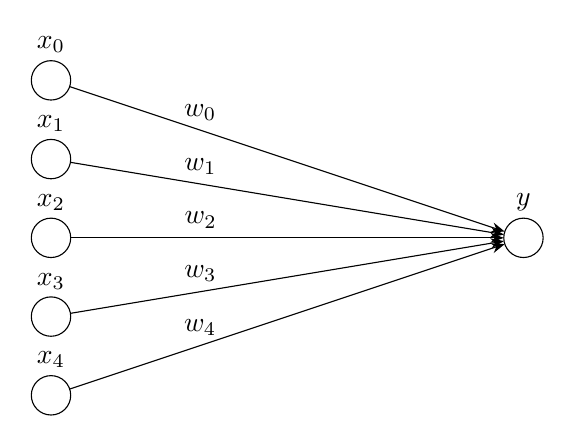
\begin{tikzpicture}
    \draw[->] (0.23717082451262844, 3.9209430584957907) to (5.762829175487371, 2.0790569415042093);
    \draw (0, 4) circle (0.25cm);
    \node at (0, 4.45) { $x_0$ };
    \node[above] at (1.8948683298050513, 3.368377223398316) { $w_0$ };
    \draw[->] (0.24659848095803594, 2.9589002531736606) to (5.753401519041964, 2.0410997468263394);
    \draw (0, 3) circle (0.25cm);
    \node at (0, 3.45) { $x_1$ };
    \node[above] at (1.8986393923832146, 2.683560101269464) { $w_1$ };
    \draw[->] (0.25, 2.0) to (5.75, 2.0);
    \draw (0, 2) circle (0.25cm);
    \node at (0, 2.45) { $x_2$ };
    \node[above] at (1.9, 2.0) { $w_2$ };
    \draw[->] (0.24659848095803594, 1.0410997468263392) to (5.753401519041964, 1.9589002531736608);
    \draw (0, 1) circle (0.25cm);
    \node at (0, 1.45) { $x_3$ };
    \node[above] at (1.8986393923832146, 1.3164398987305357) { $w_3$ };
    \draw[->] (0.23717082451262844, 0.07905694150420949) to (5.762829175487371, 1.9209430584957905);
    \draw (0, 0) circle (0.25cm);
    \node at (0, 0.45) { $x_4$ };
    \node[above] at (1.8948683298050513, 0.6316227766016838) { $w_4$ };
    \draw (6, 2) circle (0.25cm);
    \node at (6, 2.45) { $y$ };
  \end{tikzpicture}
  \end{center}
  In such a graphical representation, the set of $x_i$ nodes are called the \textbf{input layer} (or simply the first layer)
  and the $y$ node is called the \textbf{output layer}. In the above diagram, the output layer 
  consists of one node, but as we will see it can also consist of multiple nodes.

  The output is obtained as a function of the input and weights as below.
  \[
    y = \sum_{i} w_ix_i  
  \] 
  From a statistics perspective, this is actually just a \textbf{linear model}. In statistics, 
  one ``trains'' such a linear model via linear regression on some dataset. If you have 
  taken a statistics course, you might remember that this strategy works on simple 
  examples (e.g., a suspiciously-already-linear weather dataset in a Pearson textbook), 
  but linear models do not generalize and often fail to capture complex behavior.

  As we will see, neural networks are different from linear models since they add properties 
  of hidden layers and nonlinearity.
  
  \section{Hidden Layers}

  Neural networks extend our previous notion of a linear model via \textbf{hidden layers}, which can 
  be defined as one or more layers between the input and output layer. Below, we have 
  a neural network which has one hidden layer. The hidden layer can 
  have a variable number of nodes, but in our example below we have five.

  In this example, each input node $x_i$ connects to each node $h_j$ in the hidden layer 
  via a weight $w_{ij}$. These weights are illustrated by the arrows, although we are 
  choosing to suppress the $w_{ij}$ notation in the diagram below to not over complicate the figure.  
  \begin{center}
    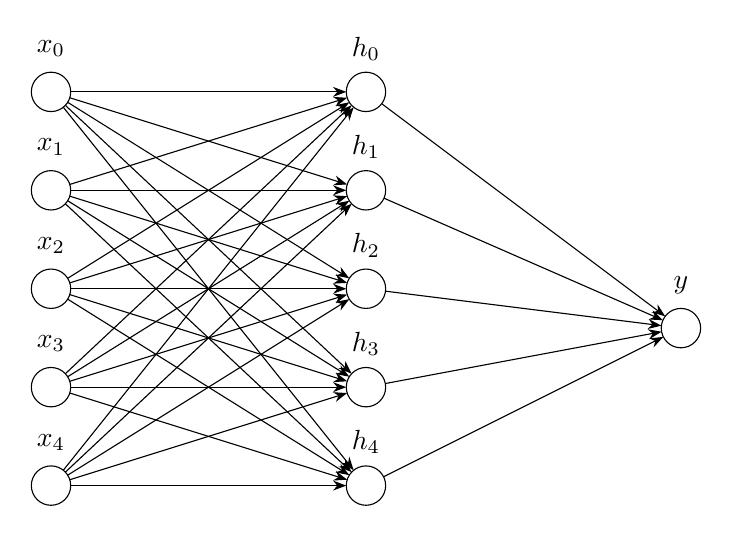
\begin{tikzpicture}
      \draw (0, 5.0) circle (0.25cm);
      \node at (0, 5.55) { $x_0$ };
      \draw (0, 3.75) circle (0.25cm);
      \node at (0, 4.3) { $x_1$ };
      \draw (0, 2.5) circle (0.25cm);
      \node at (0, 3.05) { $x_2$ };
      \draw (0, 1.25) circle (0.25cm);
      \node at (0, 1.8) { $x_3$ };
      \draw (0, 0.0) circle (0.25cm);
      \node at (0, 0.55) { $x_4$ };
      \draw (4, 5.0) circle (0.25cm);
      \node at (4, 5.55) { $h_0$ };
      \draw (4, 3.75) circle (0.25cm);
      \node at (4, 4.3) { $h_1$ };
      \draw (4, 2.5) circle (0.25cm);
      \node at (4, 3.05) { $h_2$ };
      \draw (4, 1.25) circle (0.25cm);
      \node at (4, 1.8) { $h_3$ };
      \draw (4, 0.0) circle (0.25cm);
      \node at (4, 0.55) { $h_4$ };
      \draw (8, 2) circle (0.25cm);
      \node at (8, 2.55) { $y$ };
      \draw[->] (0.25, 5.0) to (3.75, 5.0);
      \draw[->] (0.23861999450875743, 4.925431251716013) to (3.7613800054912425, 3.8245687482839865);
      \draw[->] (0.21199957600127198, 4.867500264999205) to (3.788000423998728, 2.632499735000795);
      \draw[->] (0.1823843010350213, 4.829014717779668) to (3.8176156989649788, 1.4209852822203324);
      \draw[->] (0.15617376188860607, 4.804782797639242) to (3.843826238111394, 0.19521720236075757);
      \draw[->] (0.23861999450875743, 3.8245687482839865) to (3.7613800054912425, 4.925431251716013);
      \draw[->] (0.25, 3.75) to (3.75, 3.75);
      \draw[->] (0.23861999450875743, 3.6754312517160135) to (3.7613800054912425, 2.5745687482839865);
      \draw[->] (0.21199957600127198, 3.617500264999205) to (3.788000423998728, 1.382499735000795);
      \draw[->] (0.1823843010350213, 3.5790147177796676) to (3.8176156989649788, 0.17098528222033244);
      \draw[->] (0.21199957600127198, 2.632499735000795) to (3.788000423998728, 4.867500264999205);
      \draw[->] (0.23861999450875743, 2.5745687482839865) to (3.7613800054912425, 3.6754312517160135);
      \draw[->] (0.25, 2.5) to (3.75, 2.5);
      \draw[->] (0.23861999450875743, 2.4254312517160135) to (3.7613800054912425, 1.3245687482839867);
      \draw[->] (0.21199957600127198, 2.367500264999205) to (3.788000423998728, 0.132499735000795);
      \draw[->] (0.1823843010350213, 1.4209852822203324) to (3.8176156989649788, 4.829014717779668);
      \draw[->] (0.21199957600127198, 1.382499735000795) to (3.788000423998728, 3.617500264999205);
      \draw[->] (0.23861999450875743, 1.3245687482839867) to (3.7613800054912425, 2.4254312517160135);
      \draw[->] (0.25, 1.25) to (3.75, 1.25);
      \draw[->] (0.23861999450875743, 1.1754312517160133) to (3.7613800054912425, 0.07456874828398671);
      \draw[->] (0.15617376188860607, 0.19521720236075757) to (3.843826238111394, 4.804782797639242);
      \draw[->] (0.1823843010350213, 0.17098528222033244) to (3.8176156989649788, 3.5790147177796676);
      \draw[->] (0.21199957600127198, 0.132499735000795) to (3.788000423998728, 2.367500264999205);
      \draw[->] (0.23861999450875743, 0.07456874828398671) to (3.7613800054912425, 1.1754312517160133);
      \draw[->] (0.25, -1.5308084989341915e-17) to (3.75, 1.5308084989341915e-17);
      \draw[->] (4.2, 4.85) to (7.8, 2.15);
      \draw[->] (4.229039333725547, 3.649795291495073) to (7.770960666274453, 2.100204708504927);
      \draw[->] (4.248069469178417, 2.4689913163526978) to (7.751930530821583, 2.0310086836473022);
      \draw[->] (4.245718046733581, 1.2960721337625463) to (7.754281953266419, 1.9539278662374537);
      \draw[->] (4.223606797749979, 0.11180339887498945) to (7.776393202250021, 1.8881966011250106);
    \end{tikzpicture}
  \end{center}
  The calculation of a hidden layer is simply 
  \[
      h_i = \sum_{j}w_{ij}x_i
  \]  
  Intuitively, this means that each input value $x_i$ makes a weighted contribution of $w_{ij}$ 
  to the value $h_j$. Something to observe at this point is that we can summarize the entire hidden layer 
  calculation as a matrix equation:
  \begin{align}
    \vec{h}=
    \begin{bmatrix}
      h_{1} \\
      h_{2} \\
      h_{3} \\
      h_{4} \\
      h_{5}
    \end{bmatrix}
    = \begin{bmatrix}
      \sum_{i}w_{i1}x_i \\
      \sum_{i}w_{i2}x_i \\
      \sum_{i}w_{i3}x_i \\
      \sum_{i}w_{i4}x_i \\
      \sum_{i}w_{i5}x_i \\
    \end{bmatrix}
    = \begin{bmatrix}
      w_{11} & w_{12} & w_{13} & w_{14} & w_{15} \\
      w_{21} & w_{22} & w_{23} & w_{24} & w_{25} \\
      w_{31} & w_{32} & w_{33} & w_{34} & w_{35} \\
      w_{41} & w_{42} & w_{43} & w_{44} & w_{45} \\
      w_{51} & w_{52} & w_{53} & w_{54} & w_{55} \\
    \end{bmatrix}
    \cdot
    \begin{bmatrix}
      x_{1} \\
      x_{2} \\
      x_{3} \\
      x_{4} \\
      x_{5}
    \end{bmatrix}
    = 
    W\vec{x}
  \end{align}
  This suggest the concept of a \textbf{weight matrix} $W$, which is the key to calculating the 
  hidden layer $\vec{h}$ from the input $\vec{x}$.

  As we can see, between each layer we have a matrix of weights. We can denote $U$ as the matrix of 
  the weights between the output layer and the hidden layer, so that 
  $y = U\vec{h}$. 

  Often times with neural networks it is useful to introduce a \textbf{bias} in each layer.   
  A bias is an extra node, assigned a value of 1, that we can add to a layer 
  which will be used to contribute to the calculation of the next layer. Below we illustrate the network 
  we'd obtain by adding a bias to our previous network.

  \begin{center}
    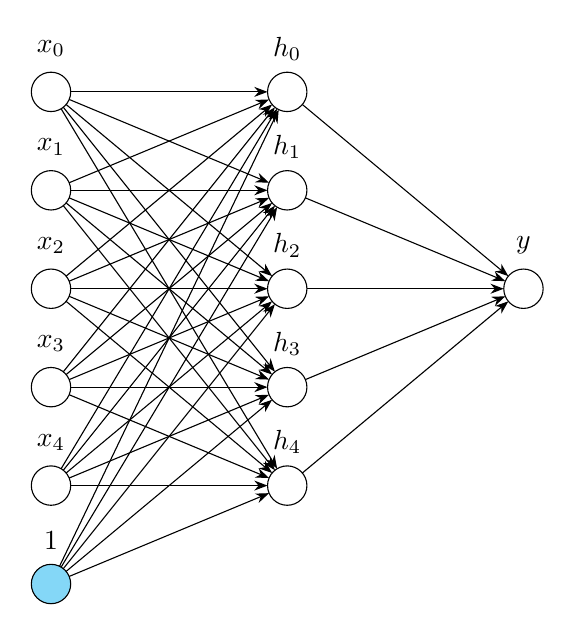
\begin{tikzpicture}
      \draw (0, 6.25) circle (0.25cm);
      \node at (0, 6.8) { $x_0$ };
      \draw (0, 5.0) circle (0.25cm);
      \node at (0, 5.55) { $x_1$ };
      \draw (0, 3.75) circle (0.25cm);
      \node at (0, 4.3) { $x_2$ };
      \draw (0, 2.5) circle (0.25cm);
      \node at (0, 3.05) { $x_3$ };
      \draw (0, 1.25) circle (0.25cm);
      \node at (0, 1.8) { $x_4$ };
      \draw[fill=ProcessBlue, fill opacity=0.5] (0, 0.0) circle (0.25cm);
      \node at (0, 0.55) { $1$ };
      \draw (3, 6.25) circle (0.25cm);
      \node at (3, 6.8) { $h_0$ };
      \draw (3, 5.0) circle (0.25cm);
      \node at (3, 5.55) { $h_1$ };
      \draw (3, 3.75) circle (0.25cm);
      \node at (3, 4.3) { $h_2$ };
      \draw (3, 2.5) circle (0.25cm);
      \node at (3, 3.05) { $h_3$ };
      \draw (3, 1.25) circle (0.25cm);
      \node at (3, 1.8) { $h_4$ };
      \draw (6, 3.75) circle (0.25cm);
      \node at (6, 4.3) { $y$ };
      \draw[->] (0.25, 6.25) to (2.75, 6.25);
      \draw[->] (0.23076923076923075, 6.153846153846154) to (2.769230769230769, 5.096153846153846);
      \draw[->] (0.19205531989934396, 6.08995390008388) to (2.8079446801006562, 3.91004609991612);
      \draw[->] (0.15617376188860607, 6.054782797639242) to (2.843826238111394, 2.6952172023607575);
      \draw[->] (0.12862393885688164, 6.035626768571864) to (2.8713760611431183, 1.4643732314281361);
      \draw[->] (0.23076923076923075, 5.096153846153846) to (2.769230769230769, 6.153846153846154);
      \draw[->] (0.25, 5.0) to (2.75, 5.0);
      \draw[->] (0.23076923076923075, 4.903846153846154) to (2.769230769230769, 3.8461538461538463);
      \draw[->] (0.19205531989934396, 4.83995390008388) to (2.8079446801006562, 2.66004609991612);
      \draw[->] (0.15617376188860607, 4.804782797639242) to (2.843826238111394, 1.4452172023607575);
      \draw[->] (0.19205531989934396, 3.91004609991612) to (2.8079446801006562, 6.08995390008388);
      \draw[->] (0.23076923076923075, 3.8461538461538463) to (2.769230769230769, 4.903846153846154);
      \draw[->] (0.25, 3.75) to (2.75, 3.75);
      \draw[->] (0.23076923076923075, 3.6538461538461537) to (2.769230769230769, 2.5961538461538463);
      \draw[->] (0.19205531989934396, 3.58995390008388) to (2.8079446801006562, 1.41004609991612);
      \draw[->] (0.15617376188860607, 2.6952172023607575) to (2.843826238111394, 6.054782797639242);
      \draw[->] (0.19205531989934396, 2.66004609991612) to (2.8079446801006562, 4.83995390008388);
      \draw[->] (0.23076923076923075, 2.5961538461538463) to (2.769230769230769, 3.6538461538461537);
      \draw[->] (0.25, 2.5) to (2.75, 2.5);
      \draw[->] (0.23076923076923075, 2.4038461538461537) to (2.769230769230769, 1.3461538461538463);
      \draw[->] (0.12862393885688164, 1.4643732314281361) to (2.8713760611431183, 6.035626768571864);
      \draw[->] (0.15617376188860607, 1.4452172023607575) to (2.843826238111394, 4.804782797639242);
      \draw[->] (0.19205531989934396, 1.41004609991612) to (2.8079446801006562, 3.58995390008388);
      \draw[->] (0.23076923076923075, 1.3461538461538463) to (2.769230769230769, 2.4038461538461537);
      \draw[->] (0.25, 1.25) to (2.75, 1.25);
      \draw[->] (0.10818276689619283, 0.2253807643670684) to (2.891817233103807, 6.024619235632931);
      \draw[->] (0.12862393885688164, 0.21437323142813605) to (2.8713760611431183, 4.785626768571864);
      \draw[->] (0.15617376188860607, 0.19521720236075757) to (2.843826238111394, 3.5547827976392425);
      \draw[->] (0.19205531989934396, 0.16004609991611995) to (2.8079446801006562, 2.33995390008388);
      \draw[->] (0.23076923076923075, 0.09615384615384617) to (2.769230769230769, 1.1538461538461537);
      \draw[->] (3.1920553198993438, 6.08995390008388) to (5.807944680100656, 3.91004609991612);
      \draw[->] (3.230769230769231, 4.903846153846154) to (5.769230769230769, 3.8461538461538463);
      \draw[->] (3.25, 3.75) to (5.75, 3.75);
      \draw[->] (3.230769230769231, 2.5961538461538463) to (5.769230769230769, 3.6538461538461537);
      \draw[->] (3.1920553198993438, 1.41004609991612) to (5.807944680100656, 3.58995390008388);
    \end{tikzpicture}
  \end{center}


  If we introduce bias in our above network, the calculation becomes 
  \[
    h_i = \sum_{j}w_{ij}x_i + b_i
  \]  
  where $b_i$ denotes the bias assigned to the hidden layer node $h_i$.  
  
  If we assemble the the bias values $b_i$ into a vector $\vec{b}$, our calculation of 
  $\vec{h}$ becomes
  \[
    \vec{h} = W\vec{x} + \vec{b}
  \]
  and if the we let $c$ (in this case, it's just a scalar instead of a vector) denote the bias in the final layer we have 
  \[
    y = U\vec{h} + c
  \]
  However, note that we're not really doing much mathematically by adding a hidden layer. 
  Observe that we can rewrite $y$ as 
  \[
      y = U\vec{h} + c = U(W\vec{x} + \vec{b}) + c = W'\vec{x} + c' 
  \]
  where $W' = UW$ and $c' = U\vec{b} + c$. This reduces our above network, with three layers, to a boring network, with two layers (similar to the one 
  we started with), just with a different weight matrix $W'$ and bias value $c'$. 
  The reason is because our network is linear, which means 
  no matter how many layers we add it will always reduce to the same boring network we started with. 
  Thus in order to get something interesting with hidden layers we need to add some nonlinearity.
  
  \section{Nonlinearity}
  Neural networks achieve our desired property of nonlinearity via usage of \textbf{activation fuctions}.
  A few common examples of such functions are the sigmoid (also known as logistic), tanh or RELU functions, and the choice of an activation 
  function depends on what one is trying to achieve with a neural network. 

  The sigmoid function is given by
  \[
      \sigma(x) = \frac{1}{1 + e^{-x}}
  \]
  The graph of the sigmoid function is given below.
  \begin{center}
    \begin{tikzpicture}
      \begin{scope}
    \draw[Gray!30, ->] (-4, 0) to (4, 0);
    \draw[Gray!30, ->] (0, 0) to (0, 5.0);
    \node[below] at (4, 0) { $x$ };
    \node[left] at (0, 5.0) { $y$ };
  \end{scope}
  
      \draw[dashed] (-3.5, 4.5) to (4.5, 4.5);
      \draw[fill] (0, 4.5) circle (0.01cm);
      \node[left] at (-3.5, 4.5) { $y=1$ };
      \draw[ProcessBlue] plot coordinates {(-4.5, 0.005262796192749818) (-4.454773869346734, 0.005631746396210898) (-4.409547738693467, 0.006026527305014147) (-4.364321608040201, 0.006448942330119109) (-4.319095477386934, 0.006900920060491525) (-4.273869346733669, 0.0073845228460029805) (-4.228643216080402, 0.007901955953416093) (-4.183417085427136, 0.008455577331464884) (-4.138190954773869, 0.009047908022967094) (-4.092964824120603, 0.009681643263881561) (-4.047738693467337, 0.01035966431124376) (-4.00251256281407, 0.011085051043962974) (-3.9572864321608043, 0.011861095382535868) (-3.9120603015075375, 0.01269131557580394) (-3.866834170854271, 0.013579471404940771) (-3.821608040201005, 0.014529580356873897) (-3.776381909547739, 0.015545934821298967) (-3.7311557788944727, 0.01663312036729784) (-3.685929648241206, 0.017796035157289784) (-3.64070351758794, 0.019039910557579216) (-3.5954773869346734, 0.020370333006064664) (-3.550251256281407, 0.02179326719867715) (-3.505025125628141, 0.02331508065675532) (-3.459798994974874, 0.024942569737754265) (-3.414572864321608, 0.026682987151332882) (-3.369346733668342, 0.0285440710418642) (-3.324120603015076, 0.030534075696637793) (-3.2788944723618094, 0.032661803936339655) (-3.2336683417085426, 0.03493664124063683) (-3.1884422110552766, 0.037368591656690056) (-3.14321608040201, 0.03996831553195919) (-3.0979899497487438, 0.04274716910453138) (-3.052763819095478, 0.0457172459741365) (-3.007537688442211, 0.04889142046473615) (-2.9623115577889445, 0.05228339287476804) (-2.9170854271356785, 0.05590773659345733) (-2.871859296482412, 0.059779947040685594) (-2.8266331658291457, 0.06391649236333043) (-2.7814070351758797, 0.06833486579230547) (-2.7361809045226133, 0.07305363953125817) (-2.690954773869347, 0.07809252000951472) (-2.6457286432160805, 0.0834724042878502) (-2.600502512562814, 0.08921543735544614) (-2.555276381909548, 0.09534506999939227) (-2.5100502512562812, 0.10188611686370903) (-2.4648241206030153, 0.10886481424252653) (-2.419597989949749, 0.11630887707120185) (-2.3743718592964824, 0.12424755448927133) (-2.329145728643216, 0.13271168324978544) (-2.28391959798995, 0.1417337381404277) (-2.2386934673366836, 0.15134787846268502) (-2.193467336683417, 0.16158998948623748) (-2.148241206030151, 0.1724977176569227) (-2.1030150753768844, 0.18411049818868822) (-2.057788944723618, 0.19646957351385033) (-2.012562814070352, 0.20961800090317478) (-1.9673366834170856, 0.2236006473998081) (-1.9221105527638191, 0.23846417004160023) (-1.8768844221105527, 0.2542569791783549) (-1.8316582914572865, 0.2710291825283369) (-1.7864321608040203, 0.2888325074673447) (-1.741206030150754, 0.30772019891019453) (-1.6959798994974875, 0.32774689003619695) (-1.650753768844221, 0.3489684430359182) (-1.605527638190955, 0.37144175702627613) (-1.5603015075376887, 0.39522454030606535) (-1.5150753768844223, 0.420375044216673) (-1.4698492462311556, 0.4469517560462967) (-1.4246231155778895, 0.4750130486842121) (-1.3793969849246233, 0.5046167851086218) (-1.334170854271357, 0.5358198762909183) (-1.2889447236180909, 0.5686777917334077) (-1.243718592964824, 0.603244022637125) (-1.1984924623115578, 0.6395694986289344) (-1.1532663316582916, 0.677701960065948) (-1.1080402010050254, 0.717685289178302) (-1.0628140703517592, 0.7595588046996393) (-1.0175879396984924, 0.803356526151213) (-0.9723618090452262, 0.8491064155640977) (-0.92713567839196, 0.8968296061080361) (-0.8819095477386938, 0.946539628797629) (-0.8366834170854276, 0.9982416501087256) (-0.7914572864321607, 1.0519317348915715) (-0.7462311557788945, 1.1075961503353762) (-0.7010050251256283, 1.1652107278379473) (-0.6557788944723622, 1.224740300377231) (-0.610552763819096, 1.2861382332838076) (-0.5653266331658291, 1.3493460660955867) (-0.5201005025125629, 1.414293282371383) (-0.4748743718592967, 1.4808972229002506) (-0.4296482412060305, 1.549063155643788) (-0.3844221105527643, 1.618684512994169) (-0.33919597989949746, 1.6896433035594725) (-0.29396984924623126, 1.7618107017739604) (-0.24874371859296507, 1.835047814283836) (-0.20351758793969887, 1.9092066174213018) (-0.158291457286432, 1.9841310553222182) (-0.11306532663316582, 2.0596582835558777) (-0.06783919597989962, 2.135620038720231) (-0.02261306532663343, 2.2118441105114752) (0.022613065326632764, 2.288155889488524) (0.06783919597989962, 2.364379961279769) (0.11306532663316582, 2.4403417164441223) (0.158291457286432, 2.515868944677782) (0.2035175879396982, 2.5907933825786973) (0.2487437185929644, 2.6649521857161633) (0.29396984924623126, 2.738189298226039) (0.33919597989949746, 2.8103566964405275) (0.38442211055276365, 2.88131548700583) (0.42964824120602985, 2.9509368443562107) (0.47487437185929604, 3.0191027770997483) (0.5201005025125629, 3.085706717628617) (0.5653266331658291, 3.1506539339044135) (0.6105527638190953, 3.2138617667161915) (0.6557788944723615, 3.275259699622768) (0.7010050251256277, 3.334789272162052) (0.7462311557788945, 3.3924038496646243) (0.7914572864321607, 3.4480682651084287) (0.8366834170854269, 3.5017583498912734) (0.8819095477386931, 3.5534603712023705) (0.9271356783919593, 3.603170393891963) (0.9723618090452262, 3.6508935844359023) (1.0175879396984924, 3.6966434738487868) (1.0628140703517586, 3.74044119530036) (1.1080402010050248, 3.782314710821697) (1.153266331658291, 3.822298039934051) (1.1984924623115578, 3.860430501371066) (1.243718592964824, 3.8967559773628744) (1.2889447236180902, 3.931322208266592) (1.3341708542713564, 3.964180123709081) (1.3793969849246226, 3.9953832148913775) (1.4246231155778895, 4.024986951315788) (1.4698492462311556, 4.053048243953704) (1.5150753768844218, 4.079624955783327) (1.5603015075376887, 4.1047754596939345) (1.6055276381909542, 4.128558242973723) (1.650753768844221, 4.1510315569640825) (1.6959798994974866, 4.172253109963803) (1.7412060301507535, 4.192279801089805) (1.7864321608040203, 4.211167492532655) (1.8316582914572859, 4.228970817471663) (1.8768844221105527, 4.245743020821645) (1.9221105527638183, 4.261535829958399) (1.9673366834170851, 4.276399352600191) (2.012562814070352, 4.290381999096825) (2.0577889447236175, 4.30353042648615) (2.1030150753768844, 4.315889501811312) (2.14824120603015, 4.327502282343077) (2.1934673366834168, 4.338410010513762) (2.2386934673366836, 4.348652121537315) (2.283919597989949, 4.358266261859572) (2.329145728643216, 4.367288316750215) (2.3743718592964815, 4.375752445510728) (2.4195979899497484, 4.3836911229287985) (2.4648241206030153, 4.391135185757473) (2.510050251256281, 4.398113883136291) (2.5552763819095476, 4.404654930000608) (2.600502512562813, 4.410784562644554) (2.64572864321608, 4.41652759571215) (2.690954773869347, 4.421907479990486) (2.7361809045226124, 4.426946360468742) (2.7814070351758793, 4.4316651342076945) (2.826633165829145, 4.4360835076366705) (2.8718592964824117, 4.440220052959314) (2.9170854271356785, 4.444092263406542) (2.962311557788944, 4.447716607125232) (3.007537688442211, 4.451108579535264) (3.0527638190954764, 4.454282754025863) (3.0979899497487433, 4.457252830895468) (3.14321608040201, 4.46003168446804) (3.1884422110552757, 4.462631408343309) (3.2336683417085426, 4.465063358759363) (3.278894472361808, 4.46733819606366) (3.324120603015075, 4.469465924303362) (3.369346733668342, 4.471455928958136) (3.4145728643216073, 4.473317012848668) (3.459798994974874, 4.475057430262245) (3.5050251256281397, 4.476684919343245) (3.5502512562814066, 4.478206732801323) (3.5954773869346734, 4.479629666993935) (3.640703517587939, 4.480960089442421) (3.685929648241206, 4.48220396484271) (3.7311557788944714, 4.483366879632702) (3.7763819095477382, 4.484454065178701) (3.821608040201005, 4.485470419643126) (3.8668341708542706, 4.486420528595058) (3.9120603015075375, 4.487308684424196) (3.957286432160803, 4.488138904617464) (4.00251256281407, 4.488914948956037) (4.047738693467337, 4.4896403356887555) (4.092964824120602, 4.490318356736118) (4.138190954773869, 4.490952091977033) (4.183417085427136, 4.491544422668535) (4.2286432160804015, 4.492098044046584) (4.273869346733669, 4.492615477153997) (4.319095477386934, 4.493099079939508) (4.364321608040201, 4.493551057669881) (4.409547738693467, 4.493973472694987) (4.454773869346733, 4.494368253603789) (4.5, 4.49473720380725) };
  \end{tikzpicture}
  \end{center}

  Using our previous network, we can add nonlinearity by defining the computation of a hidden unit to be 
  \[
    h_j = \sigma\left( \sum_{i}w_{ij}x_i + b_i \right)  
  \]
  where $\sigma$ is the activation function of choice. 

  \section{Backpropagation: A first stab}
  At this point, as we have discussed the basic properties of a neural network, 
  we will introduce a concrete example of a neural network and attempt to perform train it to 
  approximate the XOR function, which performs the following mapping on two bit inputs:
  \begin{align}
        \begin{bmatrix}
        1 \\ 0
      \end{bmatrix} \rightarrow 1 
      \hspace{1cm}
      \begin{bmatrix}
        0 \\ 0
      \end{bmatrix} \rightarrow 0
      \hspace{1cm}
      \begin{bmatrix}
        0 \\ 1
      \end{bmatrix} \rightarrow 1
      \hspace{1cm}
      \begin{bmatrix}
        1 \\ 1
      \end{bmatrix} \rightarrow 0
    \end{align}
  Below is our proposed network.
  \begin{center}
    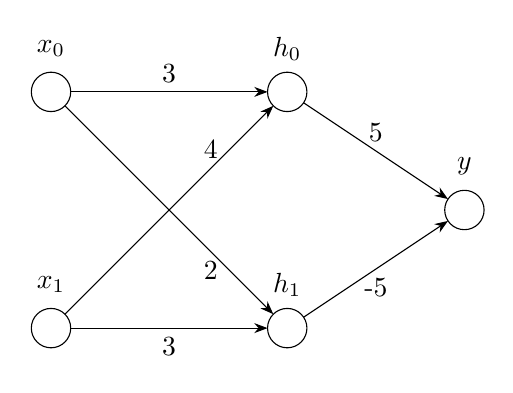
\begin{tikzpicture}
      \draw (0, 3) circle (0.25cm);
      \node at (0, 3.55) { $x_0$ };
      \draw (0, 0) circle (0.25cm);
      \node at (0, 0.55) { $x_1$ };
      \draw (3, 3) circle (0.25cm);
      \node at (3, 3.55) { $h_0$ };
      \draw (3, 0) circle (0.25cm);
      \node at (3, 0.55) { $h_1$ };
      \draw (5.25, 1.5) circle (0.25cm);
      \node at (5.25, 2.05) { $y$ };
      \draw[->] (0.25, 3.0) to (2.75, 3.0);
      \draw[->] (0.17677669529663687, 2.823223304703363) to (2.823223304703363, 0.1767766952966369);
      \draw[->] (0.17677669529663687, 0.1767766952966369) to (2.823223304703363, 2.823223304703363);
      \draw[->] (0.25, -1.5308084989341915e-17) to (2.75, 1.5308084989341915e-17);
      \draw[->] (3.208012573584461, 2.861324950943693) to (5.041987426415539, 1.6386750490563073);
      \draw[->] (3.208012573584461, 0.1386750490563073) to (5.041987426415539, 1.3613249509436927);
      \node[above] at (1.5, 3.0) { 3 };
      \node[below] at (2.029289321881345, 0.9707106781186549) { 2 };
      \node[above] at (2.029289321881345, 2.029289321881345) { 4 };
      \node[below] at (1.5, 0.0) { 3 };
      \node[above] at (4.125, 2.25) { 5 };
      \node[below] at (4.125, 0.75) { -5 };
    \end{tikzpicture}
  \end{center}
  Define the biases $\vec{b}_1$ and $\vec{b}_2$ for the first layer and the second layer, respectively, 
  to be 
  \[
    \vec{b}_1 = \begin{bmatrix}
      -2 \\ -4
    \end{bmatrix} 
    \hspace{1cm}
    \vec{b}_2 = -2 
  \]
  This leads us to define weight matrices 
  \[
    W = 
    \begin{bmatrix}
      3 & 4 \\
      2 & 3 \\
    \end{bmatrix}
    \hspace{1cm}
    U = \begin{bmatrix}
      5 & -5 \\
    \end{bmatrix}
  \]
  allowing us to write $\vec{h} = \sigma(W\vec{x} + \vec{b_1})$ and $y = \sigma(U\vec{h}) + \vec{b}_2$, or more explicitly
  \begin{align}
    h_0 = \sigma(3x_0 + 4x_1 -2)\\
    h_1 = \sigma(2x_0 + 3x_1 -4)\\
    y = \sigma(5h_1 - 5h_2 + 2)
  \end{align}
  which we can use to calculate the network.
  Below is a table of how this neural network currently computes the XOR values.
  \begin{center}
    \begin{tabular}{ |p{1.5cm}||p{3cm}|p{3cm}|p{3.5cm}|p{1.5cm}| }
      \hline
      $(x_0, x_1)$ & $h_0$ & $h_1$ & $y$ & target\\
      \hline
      $(1, 0)$ & $\sigma(1) = 0.731$ & $\sigma(-2) = 0.119$ & $\sigma(1.060) = 0.743$ & 1 \\
      \hline
      $(0, 0)$ & $\sigma(-2) = 0.119$ & $\sigma(-4) = 0.018$ & $\sigma(-1.495) = 0.183$  & 0\\
      \hline
      $(0, 1)$ & $\sigma(2) = 0.881$ & $\sigma(-1) = 0.269$ & $\sigma(1.060) = 0.743$ & 1 \\
      \hline
      $(1, 1)$ & $\sigma(5) = 0.993$ & $\sigma(1) = 0.731$ & $\sigma(-0.690) = 0.334$ & 0\\
      \hline
     \end{tabular}
     
  \end{center}
  Based on the above table, we can see that so far it's not performing that well, but after 
  all it is a first stab. This now begs the question: What does it 
  mean for a model to perform well, and how do we know when it is improving? The answer
  to this is to introduce a \textbf{cost function} which can give a measure of error. There are 
  many possible choices for a cost function, but for simplicity we will use the \textbf{least squares}
  cost function. If we have a dataset of target values $t_i$, and our model currently 
  approximates this data with a set of values $y_i$, then the measured loss is 
  \[
      L = \frac{1}{2}\sum_{i}(t_i - y_i)^2
  \]  
  The concept of a cost function now leads to the strategy of back propagation: simply change the 
  model's weights in such a way as to minimize the cost function.

  In the case of our model, we need to find out what direction, and how much, we should ``push'' each 
  value of our existing matices $U$ and $W$, so as to minimize the cost function. 
  In terms of calculus, this means we are interested in the quantities 
  \[
      \frac{dL}{du_i} \hspace{1cm} \frac{dL}{dw_{ij}}
  \]
  Once we obtain these quantities, we can update our weights after reviewing one training
  example $t_i$ via
  \begin{align}
    u'_i &= u_i - \frac{dL}{du_i} \\
    w'_{ij}  &= w_{ij} - \frac{dL}{dw_{ij}}
  \end{align}

  

  
  \section{Backpropagation: More generally}








\end{document}